\documentclass{article}
\usepackage[T1]{fontenc}
\usepackage{lmodern}
\usepackage{graphicx}
\usepackage{amsmath,amssymb}
\usepackage[a4paper,margin=2cm]{geometry}
\usepackage[absolute,overlay]{textpos}
\setlength{\TPHorizModule}{1mm}
\setlength{\TPVertModule}{1mm}
\usepackage[indonesian]{babel}
\usepackage{hyperref}
\setlength{\emergencystretch}{2em}
% unit: Halaman 13

\begin{document}

% === Halaman 13 (llm) ===

\vspace{136.62mm}

3. Yakin pengirim pesan adalah asli (authentication), bukan pihak ketiga yang menyerupai.\vspace{50mm}
\begin{center}
Dia mengklaim bahwa dia adalah $A$
\end{center}
\vspace{50mm}
4. Pengirim pesan tidak dapat menyangkal (non repudiation) telah mengirim pesan.

% deskripsi: Ilustrasi konsep autentikasi yang menunjukkan dua pihak A dan B dengan pihak ketiga di tengah yang mencoba menyerupai A.
% bbox normalisasi: [0.0380, 0.3400, 0.3800, 0.7400]
\begin{textblock*}{71.82mm}(7.98mm,100.98mm)
\noindent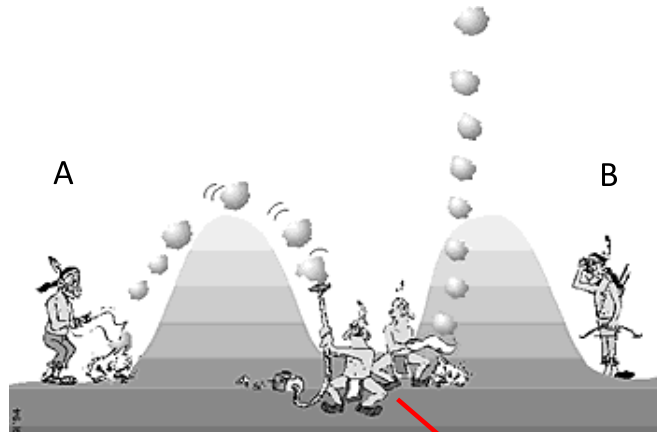
\includegraphics[width=71.82mm,height=118.80mm]{../../images/llm/page_013_img_01.png}%
\end{textblock*}

% deskripsi: Diagram konsep Non-Repudiation yang menunjukkan proses transfer dana dan penyangkalan pengiriman pesan.
% bbox normalisasi: [0.5450, 0.3600, 0.8970, 0.8200]
\begin{textblock*}{73.92mm}(114.45mm,106.92mm)
\noindent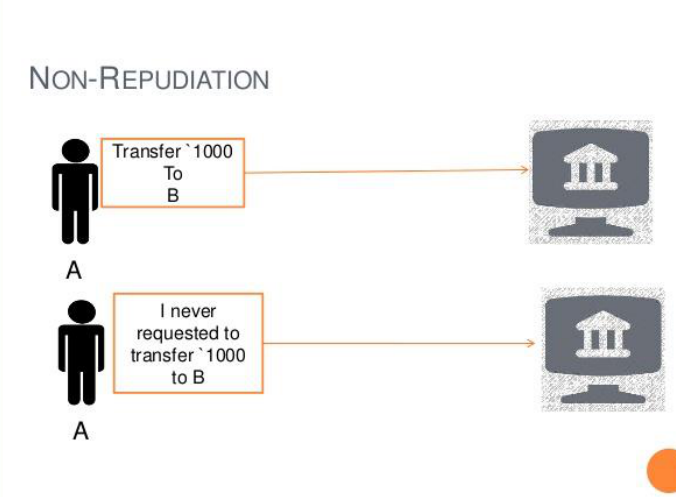
\includegraphics[width=73.92mm,height=136.62mm]{../../images/llm/page_013_img_02.png}%
\end{textblock*}

\end{document}
